% !TEX TS-program = xelatex
% !TEX encoding = UTF-8 Unicode
% !Mode:: "TeX:UTF-8"

\documentclass{resume}
\usepackage{ctex}
\usepackage{graphicx}
\usepackage{tabu}
\usepackage{multirow}
%\usepackage{zh_CN-Adobefonts_external} % Simplified Chinese Support using external fonts (./fonts/zh_CN-Adobe/)
%\usepackage{zh_CN-Adobefonts_internal} % Simplified Chinese Support using system fonts
\usepackage{linespacing_fix} % disable extra space before next section
\usepackage{cite}

\begin{document}
\pagenumbering{gobble} % suppress displaying page number

\name{\textbf{吴\ 天\ 雄}}

\Large{
	\begin{tabu}{ c l r }
		\multirow{5}{1in}{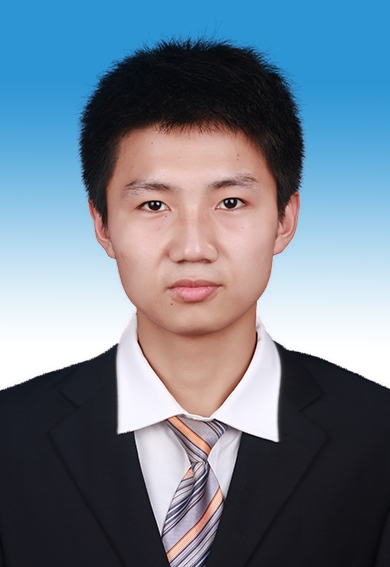
\includegraphics[width=0.88in]{wtx.jpg}} & \scshape{Tianxiong Wu} & \pbar{Java}{0.75} \\
		& \email{wutianxiong626@gmail.com} & \pbar{Scala}{0.5} \\
		& \phone{(+86) 132-8109-5873} & \pbar{Linux}{0.7} \\
		& \linkedin[Tianxiong Wu]{http://www.linkedin.com/in/tianxiong-wu-5156ba103/} & \pbar{Hadoop}{0.5} \\
		& \github[github.com/wtx626]{https://github.com/wtx626} & \pbar{Spark}{0.75}
	\end{tabu}
}
 
\section{\faGraduationCap\  \textbf{教育背景}}
\datedsubsection{\textbf{中南财经政法大学}, 武汉}{2012 -- 2016}
\textit{工学学士}\ 计算机科学与技术
\datedsubsection{\textbf{四川大学}, 成都}{2016 -- 至今}
\textit{在读硕士研究生}\ 计算机技术 

\section{\faCogs\ \textbf{所获证书}}
\begin{itemize}
  \item 四六级证书
  \item 软件设计师证书(中级)
  \item 软件著作权
\end{itemize}

\section{\faUsers\ \textbf{本科项目经历}}
\datedsubsection{\textbf{参加中南财经政法大学教务部官方安卓版APP的设计与开发} }{2014.2 -- 2014.6}
APP名称:掌上中南大,于2014年6月上线,用户量达7000。主要功能包括查看课表、成绩查询、空教室查询及一键评教。

\datedsubsection{\textbf{主持第七届全国信息安全竞赛---基于 Android 平台的远程监控系统}}{2014.4 -- 2014.7}
系统由被控端与主控端两个 APP 组成,主控端上通过发送命令,获取被控端上的相关信息。其中被控端使用到了多线程、广播进制、后台服务及安卓 rootkit技术,使其隐蔽在被控手机上;主控端使用了广播进制与多线程技术

\datedsubsection{\textbf{主持2015年度全国大学生创新训练项目并获国家级重点立项}}{2015.5 -- 2015.12}
项目为《可定制化的心理服务系统》,项目创意来源于当前大学生面对心理问题不敢于去心理咨询室寻求帮助。主要功能包括心理测试、心理美文、在线预约及匿名聊天。

\datedsubsection{\textbf{新加坡国立大学暑期实习}}{2015.7 -- 2015.8}
在NUS计算机学院选修了《计算机思维与技术》、《移动应用程序开发》。通过这两门课程的学习,我深入了解了《算法导论》的相关知识,以及安卓的游戏开发等内容。

\section{\faUsers\ \textbf{硕士研究经历}}
\datedsubsection{\textbf{研究方向}}{}
主要从事大数据研发的相关研究,优化大数据内存计算引擎Spark。

\datedsubsection{\textbf{Spark作业核心源码分析}}{2016.9 --2017.4}
完整的理清了 Spark 作业从提交到运行结束整个过程的具体流程,分析文档\url{http://wutianxiong.top/2017/10/27/Spark-Core-Source-Analyse/#more } 

\datedsubsection{\textbf{中国工程物理研究院计算机研究所(九院)网络安全大数据分析平台}}{2017.7 --2017.8}
通过对单位内流量包数据的离线和实时解析,判断单位内网络安全态势状况,大数据平台处理流量达到 7Gbps。本人在项目中负责整个网络流量的数据流pipeline的设计、搭建、实施及优化工作。

\datedsubsection{\textbf{负责大数据平台下应用程序Jar包保护}}{2017.9 --2017.11}
当大数据分析应用平台厂商需将应用程序(Java)交付给用户使用同时不希望源码泄露,此时就需要保护Java程序。本人通过使用JNI封装解密方法,定制Java类加载程序以及结合Spark和MR程序的运行原理实现了对Java程序的保护。本项目已经在实验室产品链上使用
\section{\faHeartO\ \textbf{获奖情况}}
% increase linespacing [parsep=0.5ex]
\begin{itemize}[parsep=0.5ex]
  \item 2014年获优秀学生暨二等奖学金
  \item 2015年度获优秀学生班干部暨二等奖学金
  \item 第七届全国信息安全竞赛国家级三等奖
  \item 2015年甲骨文杯全国Java程序设计大赛华中区一等奖
  \item 第六届全国大学生软件服务外包大赛国家级三等奖
  \item 2016年度中南财经政法大学优秀毕业生 
  \item 2016-2017年度四川大学优秀研究生
\end{itemize}
\section{\faInfo\ 其他}
% increase linespacing [parsep=0.5ex]
\begin{itemize}[parsep=0.5ex]
	\item 技术博客: \url{http://wutianxiong.top}
	\item GitHub: \url{https://github.com/wtx626}
	\item 语言: 英语 - 熟练
\end{itemize}
\end{document}
